183. \begin{figure}[ht!]
\center{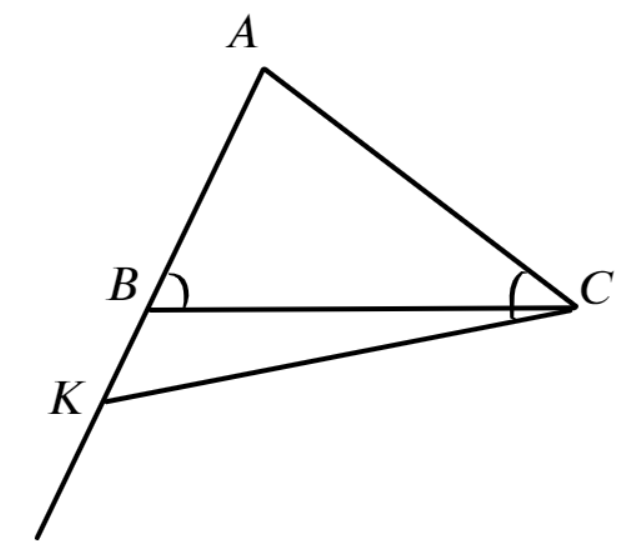
\includegraphics[scale=0.35]{g8-183.png}}
\end{figure}\\
Треугольники $ABC$ и $KAC$ подобны по двум углам $(\angle KCA = \angle ABC,$ угол $A$ --- общий). Поэтому $\cfrac{KA}{AC}=\cfrac{KC}{BC}=\cfrac{AC}{AB},$ то есть
$\cfrac{KA}{8}=\cfrac{KC}{9}=\cfrac{8}{5},$ откуда $KA=\cfrac{64}{5},\ KC=\cfrac{72}{5}.$ Тогда $KB=\cfrac{64}{5}-5=\cfrac{39}{5},\ BC=9,\ KC=\cfrac{72}{5}.$\\
